\title{Lecture 22\\Principles of Multi-Agent Knowledge Base Processing}

\begin{frame}
	\titlepage
\end{frame}

\begin{frame}{\\Lecture outline}
	\topline
	\justifying
	sc-agents and their classification. Implementing multi-agent knowledge processing in semantic memory. Specifying actions through sc-agents and solving a problem with a group of agents. The computer system user as an sc-agent. Specifying sc-agents in a knowledge base. Atomic and non-atomic sc-agents and their hierarchy.
\end{frame}

\begin{frame}{\\Logically atomic processes}
	\topline
	\justifying
	\setlength{\emergencystretch}{2em}

	\begin{textitemize}
	\item \textbf{\textit{process in sc-memory}} (sc-process) is an action or transformation performed in sc-memory by an agent or a group of agents.
	\item A \textbf{\textit{logically atomic process}} (LAP) runs \underline{independently} of whether it is part of a larger process or has preceding or succeeding processes. It is a logically coherent act of transformation, analogous to a transaction in a database management system (DBMS).
	\item The proposal is to divide all problem-solving activity within the knowledge base into \textit{logically atomic processes}.
	\end{textitemize}
\end{frame}

\begin{frame}{\\Logically atomic processes}
	\topline
	\justifying
	\vspace{3em}
	\begin{figure}[H]
		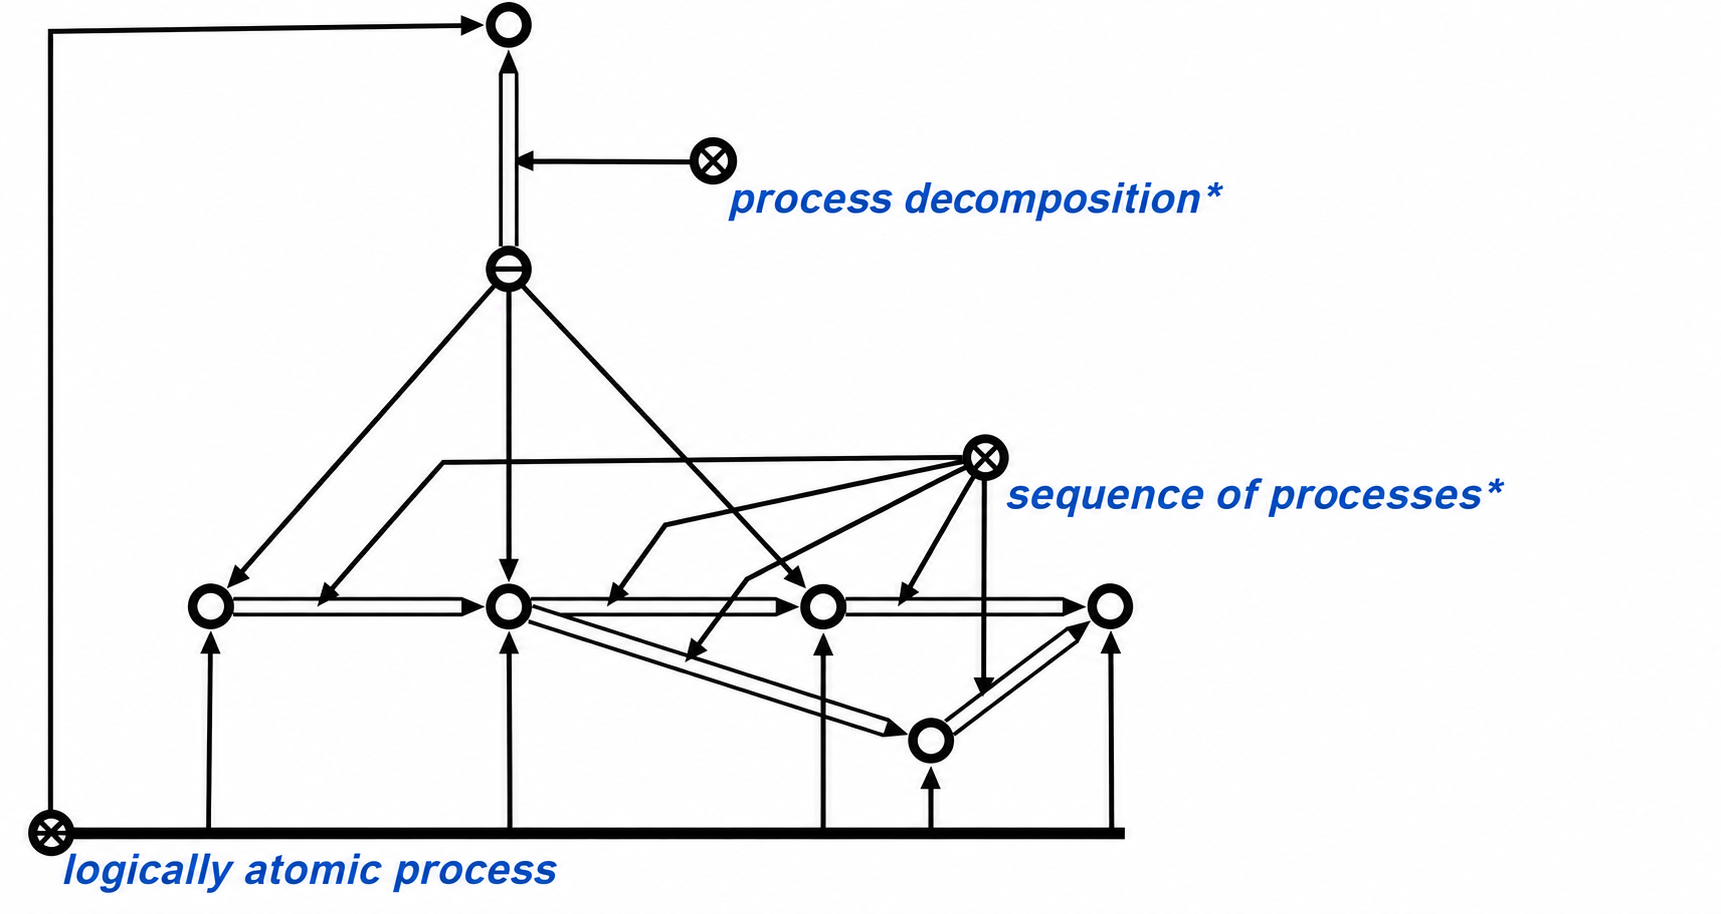
\includegraphics[width=\linewidth,height=0.68\textheight,keepaspectratio]{figures/sd_multiagent_processing/lap_en.png}
	\end{figure}
\end{frame}

\begin{frame}{\\The concept of an sc-agent}
	\topline
	\justifying

	\vspace{10mm}

	The problem solver of an OSTIS system can be divided into components called \textit{sc-agents}.

	\begin{SCn}
	\scnheader{sc-agent}
	\scnidtf{sole type of subject that performs transformations in sc-memory}
	\scnidtf{subject capable of performing actions in sc-memory that belong to a particular class of logically atomic actions}
	\end{SCn}

	The logical atomicity of an sc-agent's actions means that it responds to a corresponding class of situations or events in sc-memory and applies a specific transformation to the sc-text in the semantic neighborhood of the situation or event being processed.

\end{frame}

\begin{frame}{\\Abstract sc-agents}
		\topline
	\justifying

	Copies of the same sc-agent, or functionally equivalent sc-agents, can run in different OSTIS systems as physically distinct agents. We therefore classify and describe classes of functionally equivalent sc-agents, called \textbf{\textit{abstract sc-agents}}. Instances of such a class may be implemented in different ways.
\end{frame}


\begin{frame}{\\Specifying an abstract sc-agent}
	\topline
	\justifying
	\vspace{3em}
	\begin{figure}[H]
		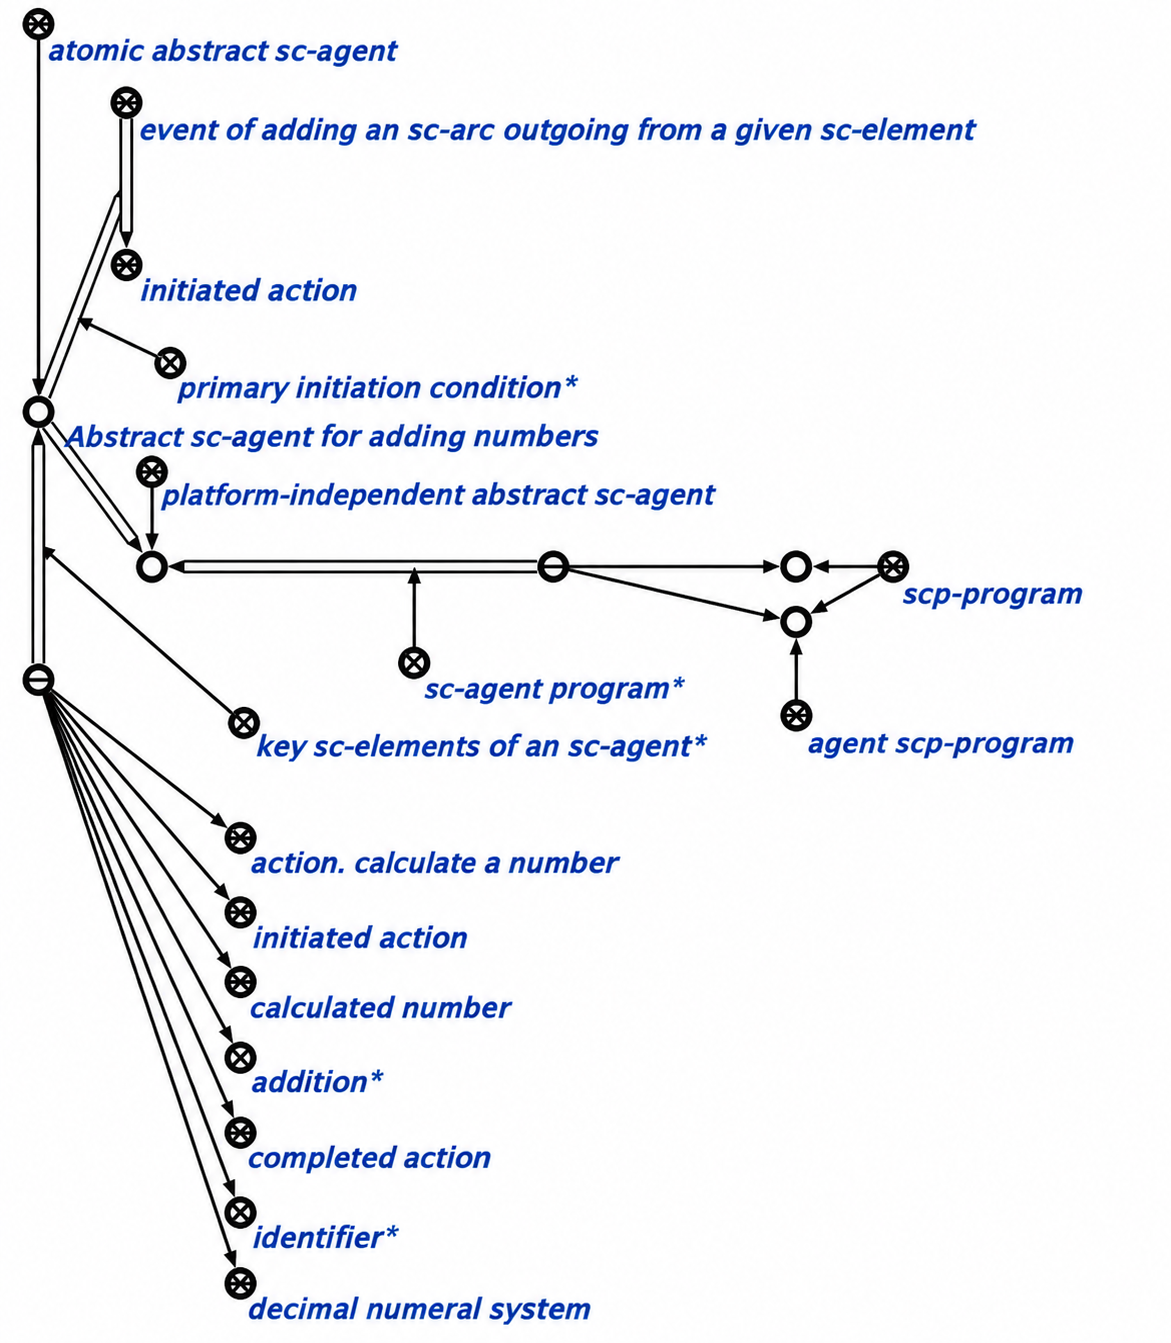
\includegraphics[width=\linewidth,height=0.71\textheight,keepaspectratio]{figures/sd_multiagent_processing/spec_en.png}
	\end{figure}
\end{frame}


\begin{frame}{sc-agent interaction: current approach}
	\topline
	\justifying
	\vspace{3em}
	\begin{figure}[H]
		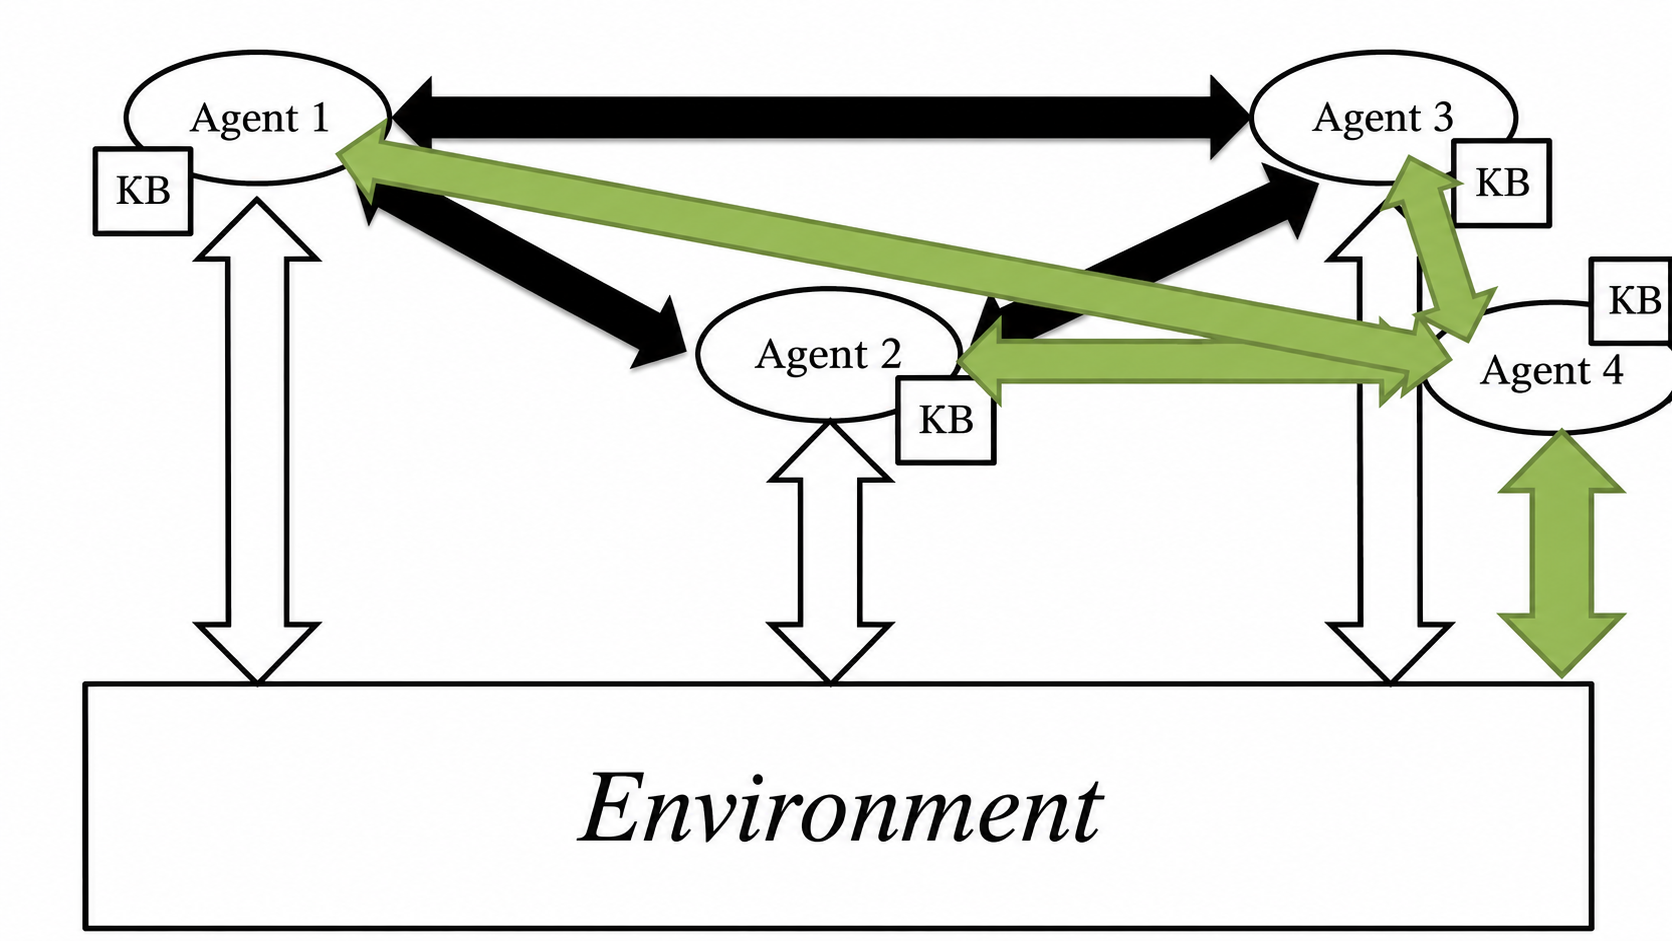
\includegraphics[width=\linewidth,height=0.68\textheight,keepaspectratio]{figures/sd_multiagent_processing/agent1_en.png}
	\end{figure}
\end{frame}

\begin{frame}{sc-agent interaction: proposed approach}
	\topline
	\justifying
	\vspace{3em}
	\begin{figure}[H]
		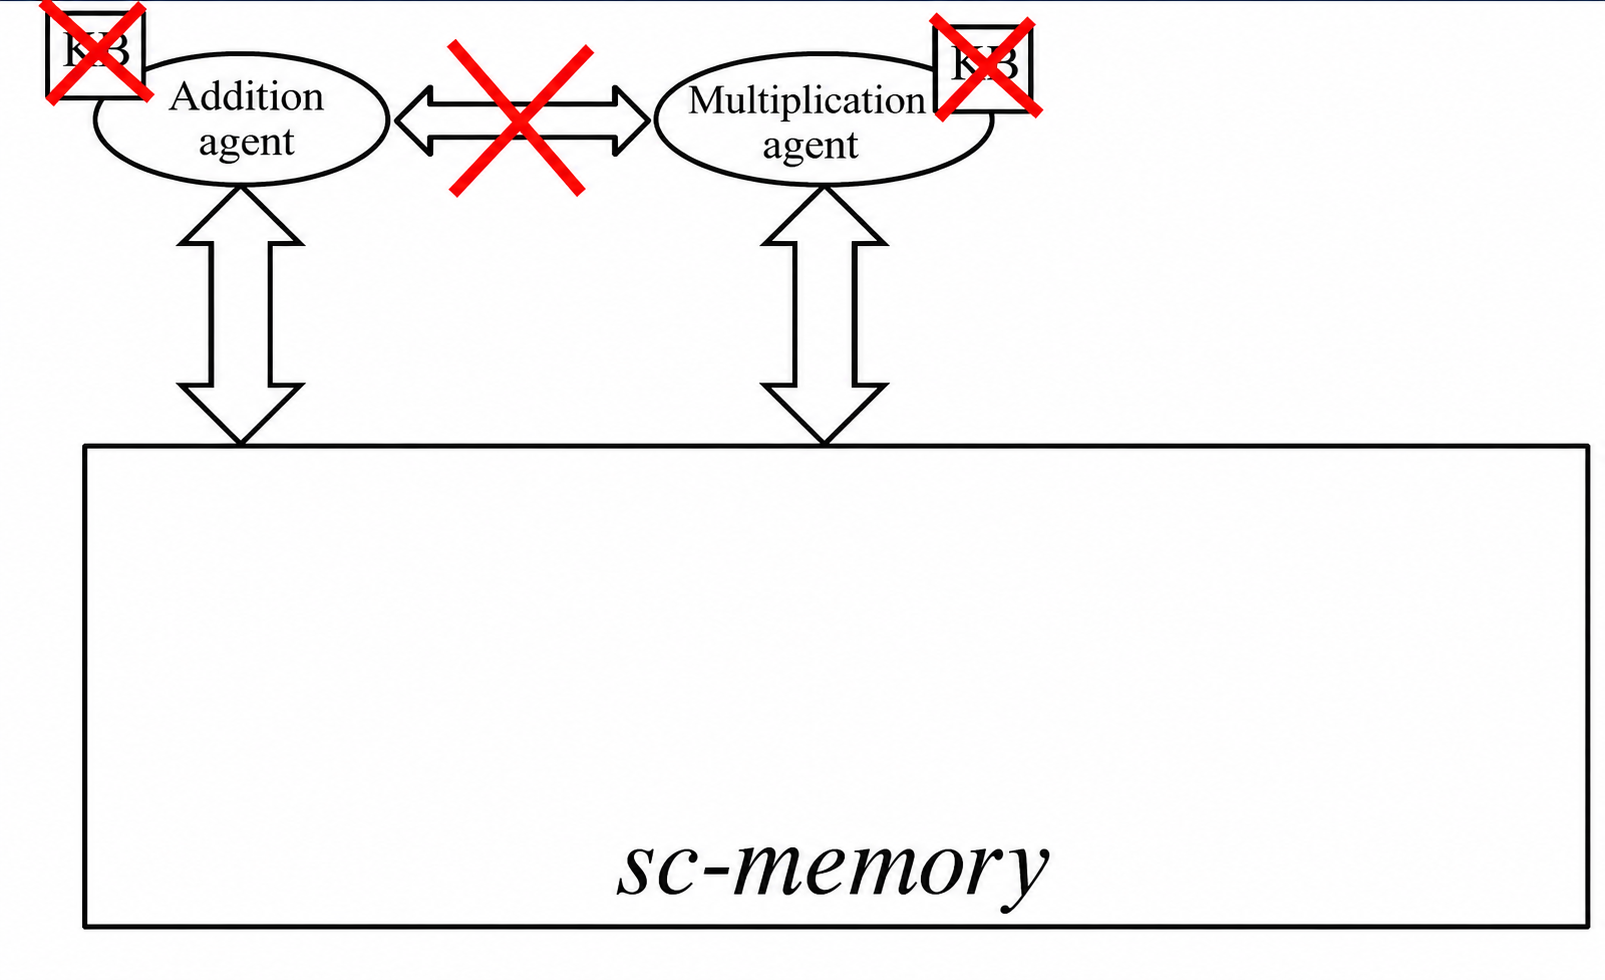
\includegraphics[width=\linewidth,height=0.68\textheight,keepaspectratio]{figures/sd_multiagent_processing/agent2_en.png}
	\end{figure}
\end{frame}

\begin{frame}{sc-agent interaction: proposed approach}
	\topline
	\justifying
	\vspace{3em}
	\begin{figure}[H]
		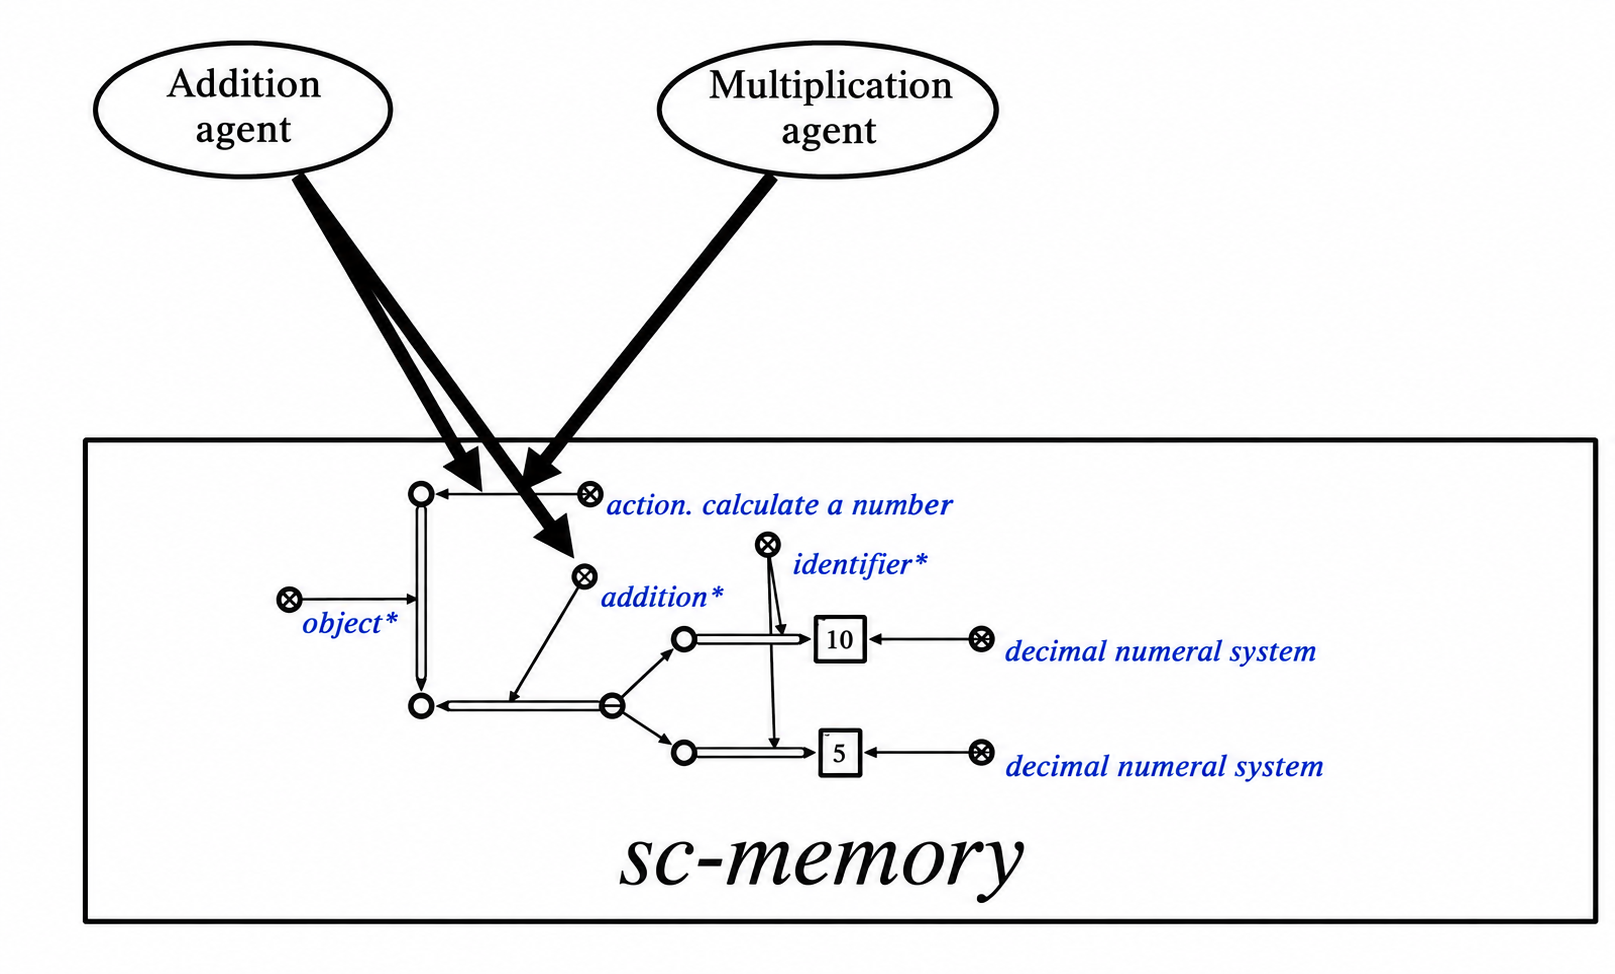
\includegraphics[width=\linewidth,height=0.68\textheight,keepaspectratio]{figures/sd_multiagent_processing/agent3_en.png}
	\end{figure}
\end{frame}

\begin{frame}{sc-agent interaction: proposed approach}
	\topline
	\justifying
	\vspace{3em}
	\begin{figure}[H]
		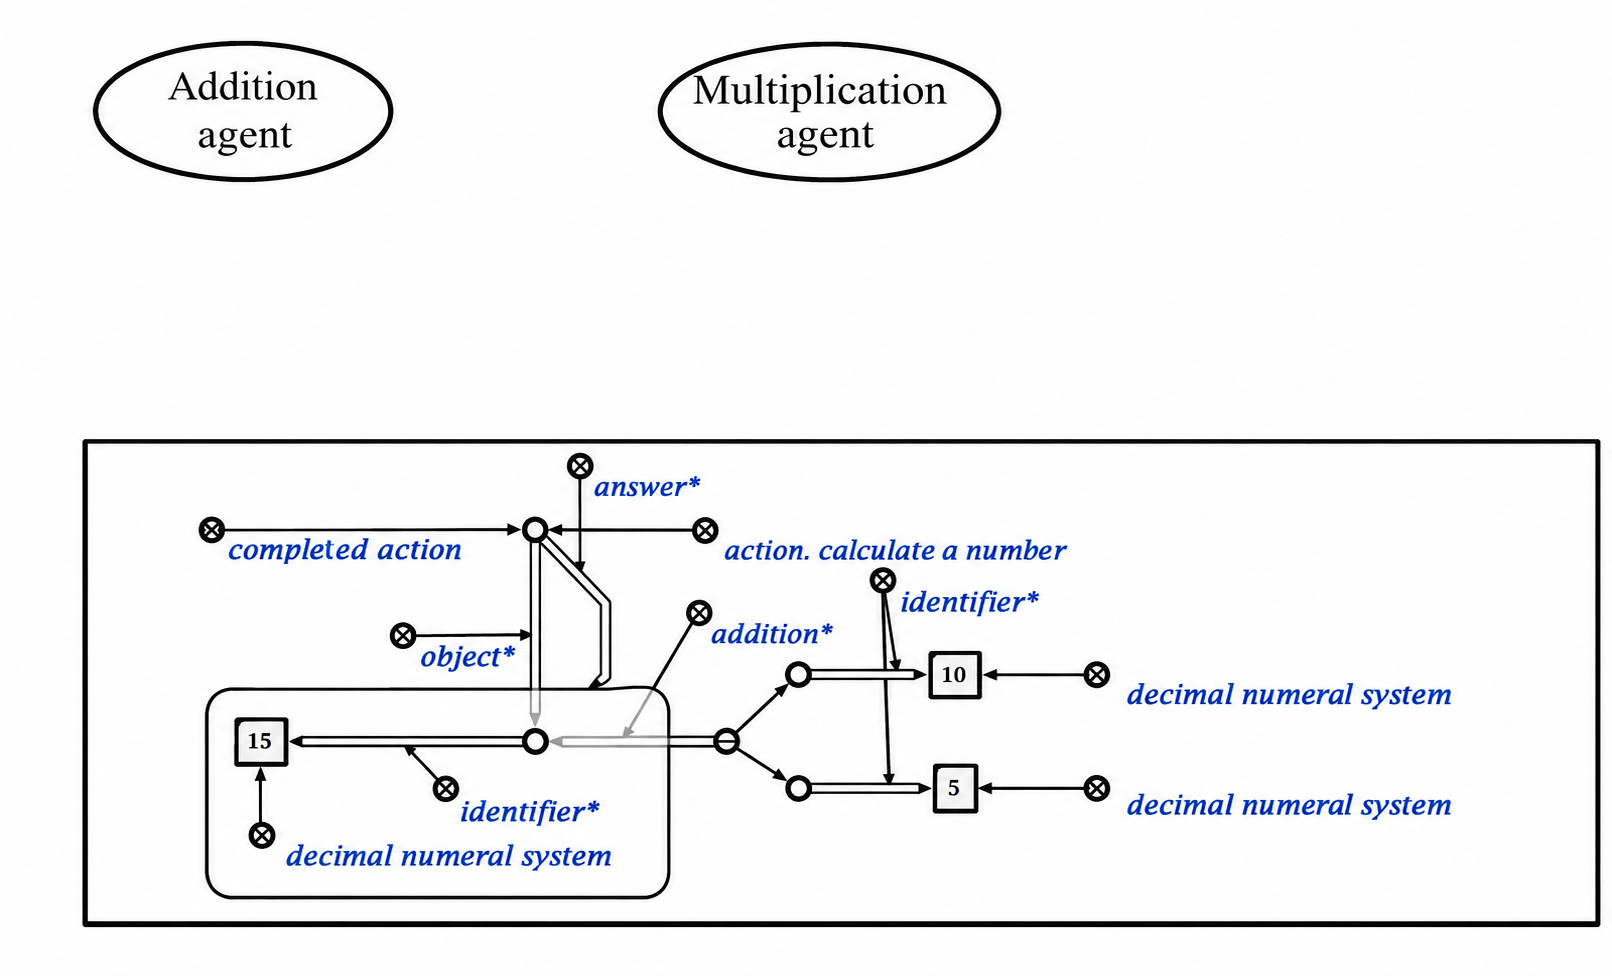
\includegraphics[width=\linewidth,height=0.68\textheight,keepaspectratio]{figures/sd_multiagent_processing/agent4_en.png}
	\end{figure}
\end{frame}

\begin{frame}{sc-agent interaction: proposed approach}
	\topline
	\justifying
	\vspace{3em}
	\begin{figure}[H]
		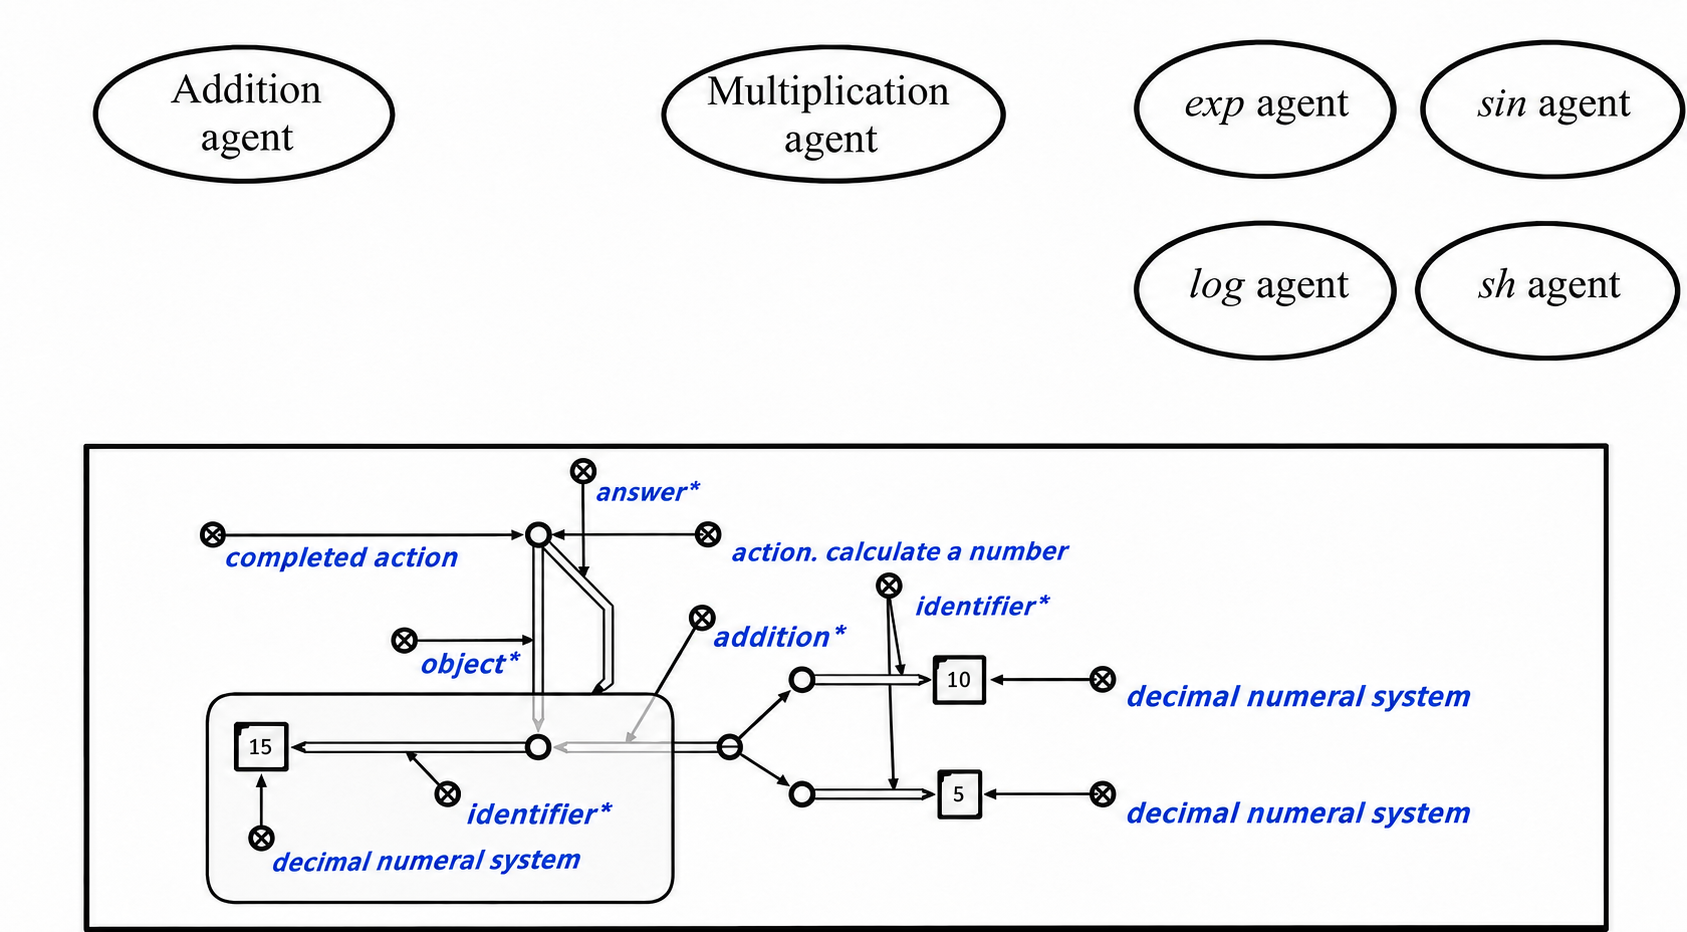
\includegraphics[width=\linewidth,height=0.68\textheight,keepaspectratio]{figures/sd_multiagent_processing/agent5_en.png}
	\end{figure}
\end{frame}

\begin{frame}{\\Classification of abstract sc-agents}
		\topline
	\justifying
	\begin{SCn}
		\scnheader{abstract sc-agent}
		\begin{scnrelfromset}{partition}
			\scnitem{non-atomic abstract sc-agent}
			\scnitem{atomic abstract sc-agent}
		\end{scnrelfromset}
		\begin{scnrelfromset}{partition}
			\scnitem{internal abstract sc-agent}
			\scnitem{effector abstract sc-agent}
			\scnitem{receptor abstract sc-agent}
		\end{scnrelfromset}
		\begin{scnrelfromset}{partition}
			\scnitem{abstract sc-agent not implementable in SCP}
			\scnitem{abstract sc-agent implementable in SCP}
		\end{scnrelfromset}
	\end{SCn}
\end{frame}
\begin{frame}{}
		\topline
	\justifying
	\begin{SCn}
		\begin{scnrelfromset}{partition}
			\scnitem{abstract sc-agent for interpreting scp-programs}
			\scnitem{abstract program sc-agent}
			\scnitem{abstract sc-meta-agent}
		\end{scnrelfromset}
		\begin{scnrelfromset}{partition}
			\scnitem{platform-dependent abstract sc-agent}
			\begin{scnindent}
				\scnsuperset{abstract sc-agent not implementable in SCP}
			\end{scnindent}
			\scnitem{platform-independent abstract sc-agent}
		\end{scnrelfromset}
	\end{SCn}
\end{frame}

\begin{frame}{\\Non-atomic abstract sc-agents}
		\topline
	\justifying
	\scnheader{non-atomic abstract sc-agent}
	\scntext{explanation}{A non-atomic abstract sc-agent is an abstract sc-agent decomposed into a group of simpler abstract sc-agents. Each may be atomic or non-atomic. In a particular alternative decomposition of the abstract sc-agent*, a non-atomic child can become an atomic abstract sc-agent and be implemented accordingly.}
\end{frame}

\begin{frame}{\\Atomic abstract sc-agents}
		\topline
	\justifying
	\scnheader{atomic abstract sc-agent}
	\scntext{explanation}{An atomic abstract sc-agent is an abstract sc-agent whose implementation platform is specified. A corresponding tuple of the sc-agent program relation exists*.}
	\begin{scnrelfromset}{partition}
		\scnitem{platform-independent atomic abstract sc-agent}
		\scnitem{platform-dependent atomic abstract sc-agent}
	\end{scnrelfromset}
\end{frame}

\begin{frame}{\\Internal abstract sc-agents}
		\topline
	\justifying
	\scnheader{internal abstract sc-agent}
	\scntext{explanation}{An internal abstract sc-agent denotes a class of sc-agents that respond to events in sc-memory and perform transformations only within that same sc-memory.}
\end{frame}

\begin{frame}{\\Effector abstract sc-agents}
		\topline
	\justifying
	\scnheader{effector abstract sc-agent}
	\scntext{explanation}{An effector abstract sc-agent denotes a class of sc-agents that respond to events in sc-memory and perform transformations in the environment outside the given OSTIS system.}
\end{frame}

\begin{frame}{\\Receptor abstract sc-agents}
		\topline
	\justifying
	\scnheader{receptor abstract sc-agent}
	\scntext{explanation}{A receptor abstract sc-agent denotes a class of sc-agents that respond to events in the environment outside an OSTIS system and perform transformations in the memory
		of that system.}
\end{frame}

\begin{frame}{sc-agents not implementable in SCP}
		\topline
	\justifying
	\scnheader{abstract sc-agent not implementable in SCP}
	\scntext{explanation}{An abstract sc-agent not implementable in SCP must be implemented on the platform that interprets sc-models, potentially in hardware. Examples are scp-program interpreters and effector and receptor abstract sc-agents.}

\end{frame}

\begin{frame}{sc-agents implementable in SCP}
		\topline
	\justifying
\scnheader{abstract sc-agent implementable in SCP}
\scntext{explanation}{An abstract sc-agent implementable in SCP can be implemented at the platform-independent level. It can also be implemented at the platform level when needed, for example to improve performance.}
\end{frame}

\begin{frame}{sc-agents for interpreting scp-programs}
		\topline
	\justifying
	\setlength{\emergencystretch}{2em}
	\scnheader{abstract sc-agent for interpreting scp-programs}
	\scntext{explanation}{These abstract sc-agents require a platform-level implementation. They interpret scp-programs and scp-metaprograms by creating scp-processes, interpreting scp-operators, and carrying out auxiliary actions. They support higher-level sc-agents implemented in SCP (program sc-agents and sc-meta-agents), including enforcing common synchronization principles.}
\end{frame}

\begin{frame}{\\Abstract program sc-agents}
		\topline
	\justifying
	\scnheader{abstract program sc-agent}
	\scntext{explanation}{Abstract program sc-agents provide the system's core functionality, enabling it to solve problems. They follow the common principles for synchronizing subjects in sc-memory.}
\end{frame}

\begin{frame}{\\Abstract sc-meta-agents}
		\topline
	\justifying
	\scnheader{abstract sc-meta-agent}
	\scntext{explanation}{Abstract sc-meta-agents coordinate abstract program sc-agents and address issues such as deadlocks. They can be implemented in SCP, but their synchronization follows different principles. They require a different level of SCP with the same types of operators and different operational semantics to account for how locks* work. We call its programs scp-metaprograms, its processes in sc-memory scp-metaprocesses, and its operators scp-metaoperators.}
\end{frame}

\begin{frame}{Platform-dependent sc-agents}
		\topline
	\justifying
	\setlength{\emergencystretch}{2em}
	\scnheader{platform-dependent abstract sc-agent}
	\scntext{explanation}{Platform-dependent abstract sc-agents are atomic abstract sc-agents implemented below the sc-model level, using a programming language other than SCP. Some sc-agents must be platform dependent, for example the interpreters of sc-models themselves and the receptor and effector agents that interact with the external environment.}
\end{frame}

\begin{frame}{Platform-independent sc-agents}
		\topline
	\justifying
	\scnheader{platform-independent abstract sc-agent}
	\scntext{explanation}{Platform-independent abstract sc-agents are atomic abstract sc-agents implemented in SCP, the basic programming language of OSTIS Technology. Platform independence here means that an atomic sc-agent implemented in SCP can be moved freely from one sc-model interpretation platform to another. Languages normally considered platform independent do not necessarily meet this OSTIS-specific definition.}
\end{frame}

\begin{frame}{Multi-agent processing in sc-memory}
		\topline
	\justifying

	A key feature of multi-agent problem solving is that different problems can be solved in parallel, which requires their information processes to run in parallel.\\
	Action in sc-memory and process in sc-memory are synonymous because every process in sc-memory is deliberate and is carried out by one or more sc-agents.\\
	Processes in sc-memory can be synchronized using a locking mechanism based on existing algorithms for synchronizing information processes in conventional systems.
\end{frame}

\begin{frame}{\\The lock relation}
	\topline
\justifying
\begin{SCn}
	\scnheader{lock relation*}
	\scniselement{binary relation}
	\scnheader{lock type}
	\scnhaselement{full lock}
	\scnhaselement{modification lock}
	\scnhaselement{deletion lock}
\end{SCn}
The lock* relation links signs of actions in sc-memory to signs of structures containing elements locked for the duration of those actions. The first component of each tuple is the sign of the action in sc-memory, and the second is the sign of the locked structure.
\end{frame}

\begin{frame}{\\Example of locks}
		\topline
	\justifying
	\vspace{3em}
	\begin{figure}[H]
		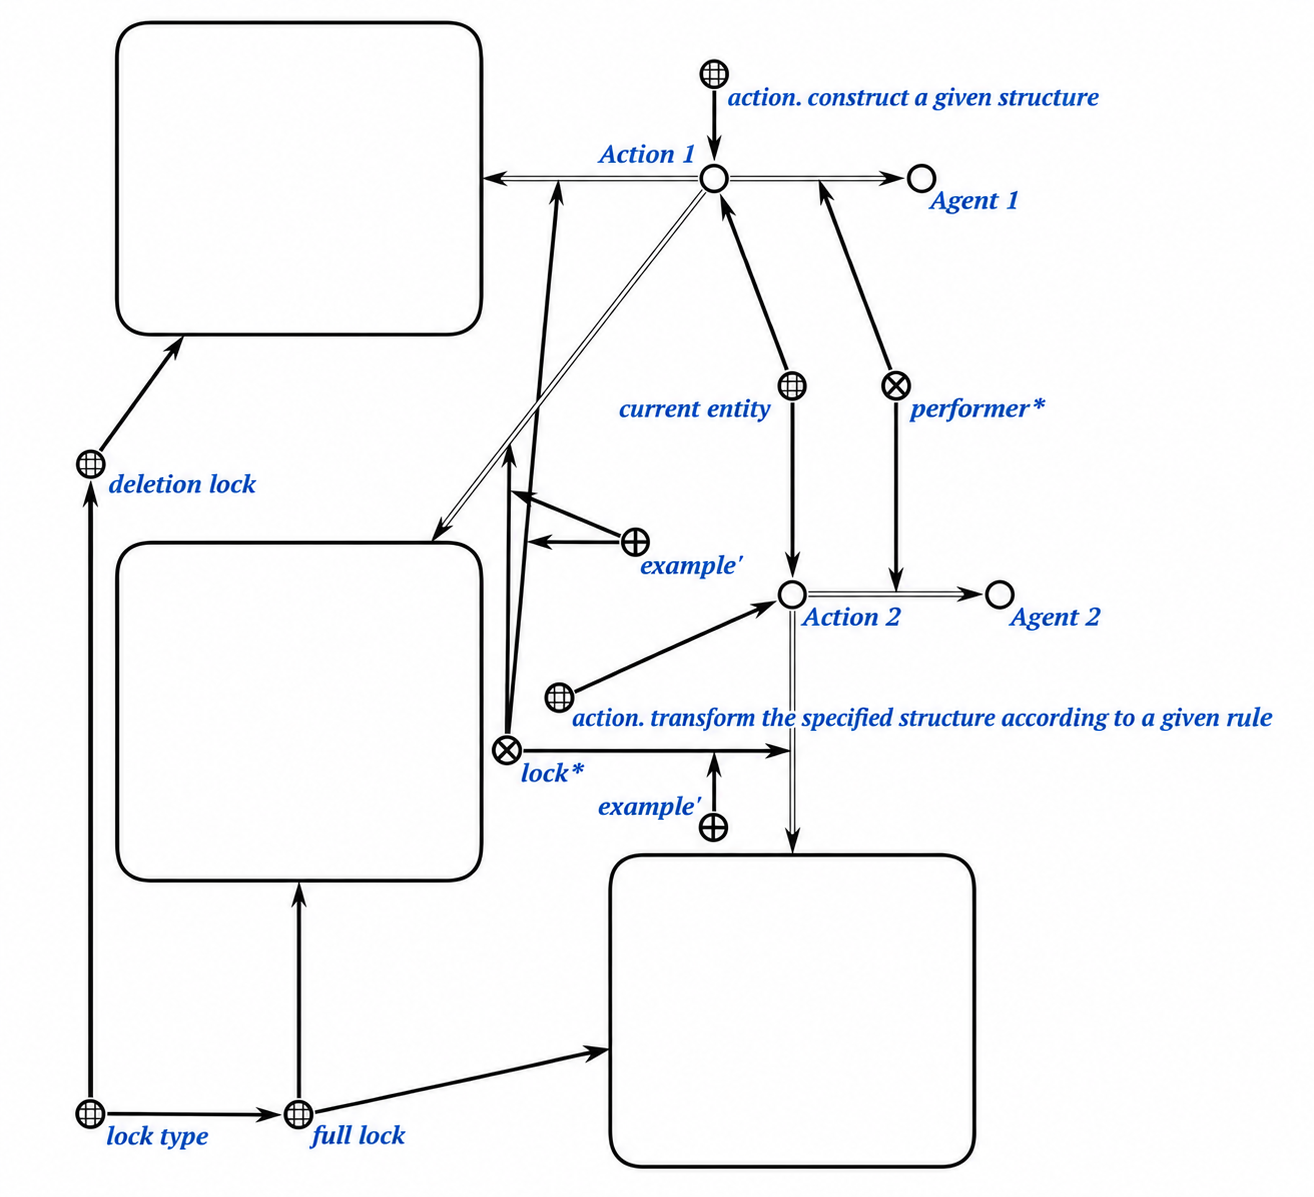
\includegraphics[width=\linewidth,height=0.71\textheight,keepaspectratio]{figures/sd_multiagent_processing/blocking_example_en.png}
	\end{figure}
\end{frame}

\begin{frame}{\\Full lock}
		\topline
	\justifying
	\begin{SCn}
		\scnheader{full lock}
		\scntext{explanation}{A structure in the full lock set contains sc-elements that only the sc-agent performing the corresponding sc-memory action can view or modify. The lock* relation connects that action to the structure. To prevent other agents from tampering with a lock, the full lock for the action also covers every element describing that lock, including the sign of the locked structure and the lock* tuples linking it to the action.}

	\end{SCn}
\end{frame}

\begin{frame}{\\Modification lock}
		\topline
	\justifying
	\begin{SCn}
		\scnheader{modification lock}
		\scntext{explanation}{A structure in the modification lock set contains sc-elements that only the agent performing the associated action can modify. The lock* relation links that action to the structure. The restriction covers physical deletion of elements or incident connectors, addition of incident sc-connectors, and changes to file contents. Any agent can still read the locked elements.}

	\end{SCn}
\end{frame}

\begin{frame}{\\Deletion lock}
		\topline
	\justifying
	\begin{SCn}
		\scnheader{deletion lock}
		\scntext{explanation}{A structure in the deletion lock set contains sc-elements that only the sc-agent performing the associated action can delete. The lock* relation links that action to the structure. Any agent can still read the elements and add incident sc-connectors.}

	\end{SCn}
\end{frame}


\begin{frame}{\\Actions specified through sc-agents}
		\topline
	\justifying
	\begin{SCn}
		\scnheader{action in sc-memory}
		\scntext{explanation}{An action in sc-memory denotes a transformation performed by an sc-agent or a group of sc-agents that changes sc-memory.}
		\scnsuperset{action in sc-memory initiated by a question}
		\scnsuperset{action to edit an OSTIS knowledge base}
		\scnsuperset{action to set the mode of an OSTIS system}
		\scnsuperset{action to edit a file stored in sc-memory}
		\scnsuperset{action to interpret a program stored in sc-memory }
	\end{SCn}
\end{frame}

\begin{frame}{The user as an sc-agent}
		\topline
	\justifying
	An OSTIS user cannot act directly in sc-memory. They can use the interface to initiate generation of an sc-text in sc-memory that specifies an action. A single atomic sc-agent can perform the action in one or several steps, or a group of sc-agents can perform it as a non-atomic agent. The specification identifies the user as the requester. In this sense the user can be regarded as an sc-agent that carries out actions in sc-memory through other agents.
\end{frame}
